\documentclass{standalone}
\usepackage{tikz}
\usetikzlibrary{patterns, positioning}


\begin{document}
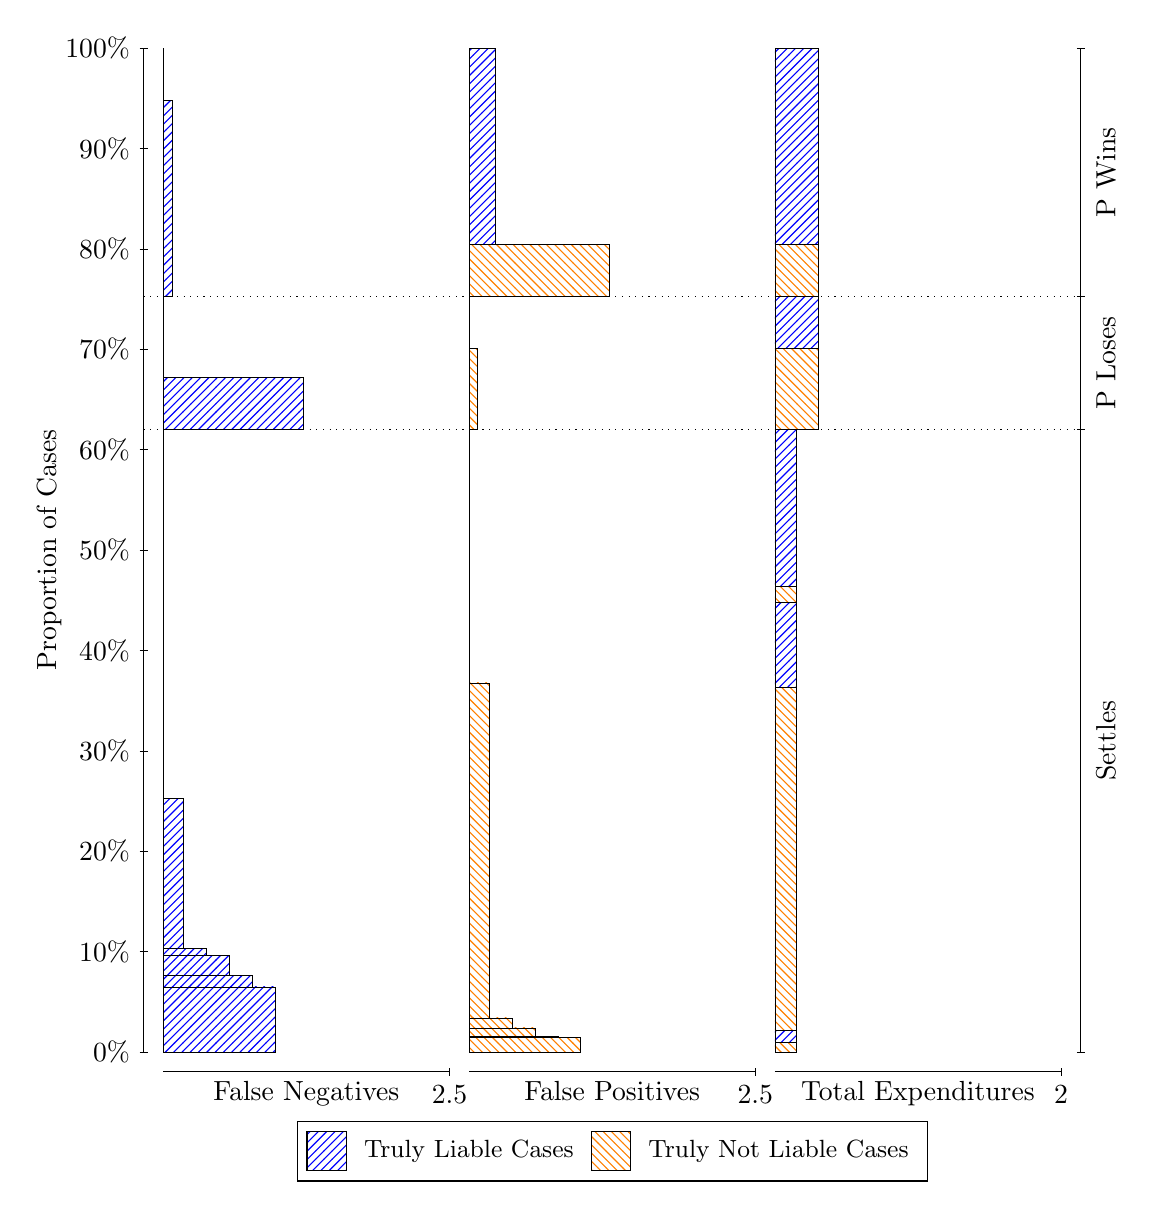
\begin{tikzpicture}
\draw[black, very thin] (1.5,1.75) -- (1.5,14.5);
\node[rotate=90, text=black, anchor=center] at (0.3, 8.125) {Proportion of Cases};
\draw[black, very thin] (1.45,1.75) -- (1.55,1.75);
\node[text=black, anchor=east] at (1.45, 1.75) {0\%};
\draw[black, very thin] (1.45,3.025) -- (1.55,3.025);
\node[text=black, anchor=east] at (1.45, 3.025) {10\%};
\draw[black, very thin] (1.45,4.3) -- (1.55,4.3);
\node[text=black, anchor=east] at (1.45, 4.3) {20\%};
\draw[black, very thin] (1.45,5.575) -- (1.55,5.575);
\node[text=black, anchor=east] at (1.45, 5.575) {30\%};
\draw[black, very thin] (1.45,6.85) -- (1.55,6.85);
\node[text=black, anchor=east] at (1.45, 6.85) {40\%};
\draw[black, very thin] (1.45,8.125) -- (1.55,8.125);
\node[text=black, anchor=east] at (1.45, 8.125) {50\%};
\draw[black, very thin] (1.45,9.4) -- (1.55,9.4);
\node[text=black, anchor=east] at (1.45, 9.4) {60\%};
\draw[black, very thin] (1.45,10.675) -- (1.55,10.675);
\node[text=black, anchor=east] at (1.45, 10.675) {70\%};
\draw[black, very thin] (1.45,11.95) -- (1.55,11.95);
\node[text=black, anchor=east] at (1.45, 11.95) {80\%};
\draw[black, very thin] (1.45,13.225) -- (1.55,13.225);
\node[text=black, anchor=east] at (1.45, 13.225) {90\%};
\draw[black, very thin] (1.45,14.5) -- (1.55,14.5);
\node[text=black, anchor=east] at (1.45, 14.5) {100\%};

\draw[black, very thin] (13.4,1.75) -- (13.4,14.5);
\draw[black, very thin] (13.35,1.75) -- (13.45,1.75);
\node[anchor=west] at (13.35, 1.75) {};
\draw[black, very thin] (13.35,9.6583) -- (13.45,9.6583);
\node[anchor=west] at (13.35, 9.6583) {};
\draw[black, very thin] (13.35,11.341) -- (13.45,11.341);
\node[anchor=west] at (13.35, 11.341) {};
\draw[black, very thin] (13.35,14.5) -- (13.45,14.5);
\node[anchor=west] at (13.35, 14.5) {};

\draw[black, very thin, pattern color=blue, pattern=north east lines] (1.75,1.75) rectangle (3.167,2.577);
\draw[black, very thin, pattern color=blue, pattern=north east lines] (1.75,2.577) rectangle (2.8763,2.7222);
\draw[black, very thin, pattern color=blue, pattern=north east lines] (1.75,2.7222) rectangle (2.5857,2.9729);
\draw[black, very thin, pattern color=blue, pattern=north east lines] (1.75,2.9729) rectangle (2.295,3.0703);
\draw[black, very thin, pattern color=blue, pattern=north east lines] (1.75,3.0703) rectangle (2.0043,4.9723);
\draw[black, very thin, pattern color=orange, pattern=north west lines] (1.75,4.9723) rectangle (1.75,9.6583);
\draw[black, very thin, pattern color=blue, pattern=north east lines] (1.75,9.6583) rectangle (3.5303,10.313);
\draw[black, very thin, pattern color=orange, pattern=north west lines] (1.75,10.313) rectangle (1.75,11.341);
\draw[black, very thin, pattern color=blue, pattern=north east lines] (1.75,11.341) rectangle (1.859,13.839);
\draw[black, very thin, pattern color=orange, pattern=north west lines] (1.75,13.839) rectangle (1.75,14.5);
\draw[black, very thin, pattern color=orange, pattern=north west lines] (5.6333,1.75) rectangle (7.0503,1.9309);
\draw[black, very thin, pattern color=orange, pattern=north west lines] (5.6333,1.9309) rectangle (6.7597,1.9513);
\draw[black, very thin, pattern color=orange, pattern=north west lines] (5.6333,1.9513) rectangle (6.469,2.0573);
\draw[black, very thin, pattern color=orange, pattern=north west lines] (5.6333,2.0573) rectangle (6.1783,2.183);
\draw[black, very thin, pattern color=orange, pattern=north west lines] (5.6333,2.183) rectangle (5.8877,6.436);
\draw[black, very thin, pattern color=blue, pattern=north east lines] (5.6333,6.436) rectangle (5.6333,9.6583);
\draw[black, very thin, pattern color=orange, pattern=north west lines] (5.6333,9.6583) rectangle (5.7423,10.686);
\draw[black, very thin, pattern color=blue, pattern=north east lines] (5.6333,10.686) rectangle (5.6333,11.341);
\draw[black, very thin, pattern color=orange, pattern=north west lines] (5.6333,11.341) rectangle (7.4137,12.002);
\draw[black, very thin, pattern color=blue, pattern=north east lines] (5.6333,12.002) rectangle (5.9603,14.5);
\draw[black, very thin, pattern color=orange, pattern=north west lines] (9.5167,1.75) rectangle (9.7892,1.8757);
\draw[black, very thin, pattern color=blue, pattern=north east lines] (9.5167,1.8757) rectangle (9.7892,2.0209);
\draw[black, very thin, pattern color=orange, pattern=north west lines] (9.5167,2.0209) rectangle (9.7892,6.3798);
\draw[black, very thin, pattern color=blue, pattern=north east lines] (9.5167,6.3798) rectangle (9.7892,7.4576);
\draw[black, very thin, pattern color=orange, pattern=north west lines] (9.5167,7.4576) rectangle (9.7892,7.6589);
\draw[black, very thin, pattern color=blue, pattern=north east lines] (9.5167,7.6589) rectangle (9.7892,9.6583);
\draw[black, very thin, pattern color=orange, pattern=north west lines] (9.5167,9.6583) rectangle (10.062,10.686);
\draw[black, very thin, pattern color=blue, pattern=north east lines] (9.5167,10.686) rectangle (10.062,11.341);
\draw[black, very thin, pattern color=orange, pattern=north west lines] (9.5167,11.341) rectangle (10.062,12.002);
\draw[black, very thin, pattern color=blue, pattern=north east lines] (9.5167,12.002) rectangle (10.062,14.5);
\draw[black, dotted] (1.5,9.6583) -- (13.4,9.6583);
\draw[black, dotted] (1.5,11.341) -- (13.4,11.341);
\draw[black, very thin] (1.75,1.5) -- (5.3833,1.5);
\node[text=black, anchor=north] at (3.5667, 1.5) {False Negatives};
\draw[black, very thin] (5.3833,1.45) -- (5.3833,1.55);
\node[text=black, anchor=north] at (5.3833, 1.45) {2.5};

\draw[black, very thin] (5.6333,1.5) -- (9.2667,1.5);
\node[text=black, anchor=north] at (7.45, 1.5) {False Positives};
\draw[black, very thin] (9.2667,1.45) -- (9.2667,1.55);
\node[text=black, anchor=north] at (9.2667, 1.45) {2.5};

\draw[black, very thin] (9.5167,1.5) -- (13.15,1.5);
\node[text=black, anchor=north] at (11.333, 1.5) {Total Expenditures};
\draw[black, very thin] (13.15,1.45) -- (13.15,1.55);
\node[text=black, anchor=north] at (13.15, 1.45) {2};

\node[text=black, centered, rotate=90] at (13.72, 5.7041) {Settles};
\node[text=black, centered, rotate=90] at (13.72, 10.499) {P Loses};
\node[text=black, centered, rotate=90] at (13.72, 12.92) {P Wins};

\draw (7.449999999999999,1.5) node[draw=none] (baseCoordinate) {};
\begin{scope}[align=center]
        \matrix[scale=0.5, draw=black, below=0.5cm of baseCoordinate, nodes={draw}, column sep=0.1cm]{
            \node[rectangle, draw, minimum width=0.5cm, minimum height=0.5cm, pattern color=blue, pattern=north east lines] {}; &
            \node[draw=none, font=\small, text=black] (B) {Truly Liable Cases}; &
            \node[rectangle, draw, minimum width=0.5cm, minimum height=0.5cm, pattern color=orange, pattern=north west lines] {}; &
            \node[draw=none, font=\small, text=black] (B) {Truly Not Liable Cases}; \\
            };
\end{scope}

\end{tikzpicture}
\end{document}